%  $Description: Author guidelines and sample document in LaTeX 2.09$
%
%  $Author: ienne $
%  $Date: 1995/09/15 15:20:59 $
%  $Revision: 1.4 $
%
%\documentclass[times, 10pt,twocolumn]{article}
\documentclass[conference,final]{IEEEtran}
\usepackage{latex8}
\usepackage{times}

% Users' option
\usepackage{amssymb}
\usepackage{amsmath}
\usepackage{graphicx}
\usepackage{epstopdf}
\usepackage{color}
\topmargin=0.01in
\usepackage{multirow}
\usepackage{booktabs}
\newif\ifdraft
\drafttrue

\renewcommand{\multirowsetup}{\centering}
\renewcommand{\arraystretch}{1.2}
\def\nyc{\centering}

\ifdraft
\newcommand{\fixme}[1]{ { \bf{ ***FIXME: #1 }} }
\newcommand{\jhanote}[1]{ {\textcolor{red} { ***Jha: #1 }}}
\newcommand{\Nkimnote}[1]{ {\textcolor{green} { ***Nkim: #1 }}}
\newcommand{\skonote}[1]{ {\textcolor{blue} { ***Jeff: #1 }}}
\newcommand{\athotanote}[1]{ {\textcolor{green} { ***athota: #1 }}}
\newcommand{\Jkimnote}[1]{ {\textcolor{red} { ***Jkim: #1 }}}
\newcommand{\yyenote}[1]{ {\textcolor{blue} { ***yye00: #1 }}}
\else
\newcommand{\jhanote}[1]{}
\newcommand{\Nkimnote}[1]{}
\newcommand{\fixme}[1]{}
\newcommand{\skonote}[1]{}
\newcommand{\Jkimnote}[1]{}
\fi
% End of users' option

%\documentstyle[times,art10,twocolumn,latex8]{article}

%-------------------------------------------------------------------------
% take the % away on next line to produce the final camera-ready version
\pagestyle{empty}

\newcommand{\up}{\vspace*{-1em}}
\newcommand{\upp}{\vspace*{-0.5em}}
\newcommand{\ts}{$T_{s}$}


%-------------------------------------------------------------------------
\title{Efficient Runtime Environment for Coupled Multi-Physics Simulations: \\
Dynamic Resource Allocation and Load-Balancing}

% \author{Soon-Heum Ko, Nayong Kim, Joohyun Kim, Abhinav Thota, Shantenu Jha\\
% Center for Computation and Technology\\
% Louisiana State University, Baton Rouge, LA 70803, USA\\
% (sko,nykim,jhkim,athota1,sjha)@cct.lsu.edu\\
% % For a paper whose authors are all at the same institution,
% % omit the following lines up until the closing ``}''.
% % Additional authors and addresses can be added with ``\and'',
% % just like the second author.
% %\and
% % Dimitris Nikitopoulos\\
% % Mechanical Engineering Department\\
% % Louisiana State University, Baton Rouge, LA 70803, USA\\
% % meniki@lsu.edu\\
% \and
% Yaakoub El Khamra\\
% Texas Advanced Computing Center\\
% The University of Texas at Austin, Austin, Texas 78758, USA\\
% yye00@austin.mail.address\\
% }

\author{
 ~\\[-2em]
 Soon-Heum Ko$^{1}$, Nayong Kim$^{1}$, Joohyun Kim$^{1}$, \\ Abhinav Thota$^{1,2}$, Shantenu Jha$^{*1,2}$\\
 \small{\emph{$^{1}$Center for Computation \& Technology, Louisiana State University, USA}}\\
 \small{\emph{$^{2}$Department of Computer Science, Louisiana State University, USA}}\\
 \small{\emph{$^{*}$Contact Author}}\\
}

%\thispagestyle{empty}

\begin{document}

\maketitle

\begin{abstract}
  Coupled Multi-Physics simulations, such as hybrid CFD-MD
  simulations, represent an increasingly important class of scientific
  applications.  Often the physical problems of interest demand the
  use of high-end computers, such as TeraGrid resources, which are
  often accessible only via batch-queues. Batch-queue systems are not
  natively developed to support the coordinated scheduling of jobs --
  which in turn is required to support the concurrent execution
  required by coupled multi-physics simulations. In this paper we
  develop and demonstrate a novel approach to overcome the lack of
  native support for coordinated job submission requirement associated
  with coupled runs. We establish the performance advantages arising
  from our solution, which is a generalization of the Pilot-Job
  concept -- which in of itself is not new, but is applied to coupled
  simulations for the first time.  Our solution not only overcomes the
  initial co-scheduling problem, but provides a dynamic resource
  allocation mechanism. Support for such dynamic resources is critical
  for a load-balancing mechanism, which we develop and demonstrate to
  be effective at reducing the total time-to-solution of the
  problem. We establish that the performance advantage of using
  BigJobs is invariant with the size of the machine as well as the
  size of the physical model under investigation.  The Pilot-Job
  abstraction is developed using SAGA, which provides an
  infrastructure agnostic implementation, and which can seamlessly
  execute and utilize distributed resources. 
\end{abstract}
\up\up


%-------------------------------------------------------------------------
\section{Introduction}

Coupled Multi-Physics simulation techniques are being increasingly
used to study many different physical phenomenon spanning time and
length scales at different level of
details~\cite{Tai}~\cite{Watanabe}. These techniques have been used to
investigate phenomena from crack-propagation in materials, biological
systems as well as understanding multi-phase fluid flow in constrained
geometry.

In addition to the ``physics challenges'' of these Multi-Physics
coupled simulations, there exist interesting ``computational
challenges''. Probably the best known (and investigated) is the
challenge of simulating large and complex systems, leading to
simulations that require greater computational resources -- often
involving HPC resources. % and no longer working on dedicated PCs.
Parallelization helps individual codes address the computational
demand of large and complex systems, but incorporating two distinct
codes under the umbrella of a single tightly-coupled application (say
using MPI) is not without significant problems. For example, the two
codes can often have very different computational kernels (one could
be mesh-based, the other unstructured particle simulations) with very
different computational time-scales.

Here we will focus on the challenges arising from running
tightly-coupled simulations on production systems with batch-queues,
whereby it cannot be guaranteed that two separate jobs will execute
concurrently. Specifically we will consider the case of coupling a
Computational Fluid Dynamics (CFD) code and a Molecular Dynamics (MD)
code, where the communication is via the exchange of files and not
Unix pipes (see next section for details on the coupling).

% Users' account loss is inevitable in conventional queuing systems
% except when sufficient CPUs are idling,

Although not exactly tightly-coupled in the sense of MPI, viz., very
frequent and with an extreme sensitivity to latency in communication
delay, the CFD and MD codes communicate frequently, (e.g., the CFD
code conducts data exchange in every iteration) and thus they need to
run concurrently. Thus, without explicit support for co-scheduling, it
is unlikely that coupled CFD-MD simulations will run concurrently as
inevitably the first job to run will have to wait for the other to
follow.

% \jhanote{Place the following appropriately} Thus, the best way using
% conventional job submission system would be to find a site with
% sufficient resource pool and submit two jobs with the optimal number
% of processors according to the pre-test data on performance of each
% tool in that facility with the same problem size.

Another important challenge, especially for large-scale simulations is
the need for efficient load-balancing, taking into account the
individual application's performance. Even if the two simulations could
run concurrently, without explicit load-management/balancing support,
there is likely to be inefficient utilization of compute resources due
to load imbalance. As the performance of each simulation component
changes with computing resource and problem size, re-adjustment of
allocated resources to each task according to their performance is
required during the simulation. Interestingly, as we will show,
effective load-balancing of two independent but concurrently running
codes introduces the need for dynamic resource allocation, and the
same solution that we devise to overcome the concurrent scheduling
requirement/constraints of coupled jobs also supports the feature of
dynamic resource allocation. In contrast, if simulations were
submitted as independent jobs, changing resource (CPU) allocation to
address these changes is challenging -- as the change in resource
assigned to one is correlated with a change in resource assigned to
the other component.

The pilot-job is just a container task where a number of sub-tasks can
run in pre-defined schedule with the specified number of processors
whether or not they are coupled.  The dynamical resource allocation
capabilties of the Pilot-Job prove useful in the other two scenarios,
as well as when using load-balancing in the single-resource scenario.
Although the container-Job/Pilot-Job concept is not novel {\it per
  se}, we believe this is the first documented utilization of these
abstractions to perform coupled Multi-Physics simulations. We claim
that there several distinct advantages that arise as a consequence of
using Pilot-Jobs for Coupled Simulations: (i) obviates the need for a
o-scheduler while preserving performance, (ii) enables dynamic
resource allocation, which in turn is important for load-balancing
across coupled simulations.  But given the lack of system or
service-level support to address the challenges outlined above, there
is a need to address the solution at the application level. This paper
aims to provide novel solutions to the above problem using frameworks
that are in user (application) space.
 
We will provide details on how we implement our solution in Section 3,
but in a nutshell it is critical to mention that our solution and its
concomittant efficiency is not tied to either a specific application
set (or infrastructure) and is scalable and extensible. It is based
upon the SAGA (the Simple API for Grid Applications)~\cite{saga_web},
which is a high-level API which provides the basic functionality
required to implement distributed functionally -- both logically and
physically, in an infrastructure and middleware independent
fashion. SAGA enables the creation of higher-levels of abstractions,
for example a container-job and pilot-job (which as we will discuss is
referred to as the BigJob~\cite{saga_royalsoc}). The SAGA-based
Pilot-Job is infrastructure neutral, unlike {\it all} other
Pilot-Jobs.

We begin the next section with an outline of the basic motivation for
coupled simulations and load balancing.  We will address the
fundamental question: Does the use of an infrastructure independent
container job assist in the time to solution of coupled simulation? We
will determine that the answer is yes for a variety of different
resource utilization scenarios. In the simplest case of a coupled
simulation running on a single machine, we will establish that the
reason is the lowered waiting time typically associated with a larger
size request (on most queuing systems, for most commonly occuring load
factors).  As our experiments will show, performance improvement arise
from removing the need for scheduling the two-components separately
and in providing a single job-requirement to the queuing system.

%\jhanote{Next few paragraphs need attention}

%\skonote{Please leave unchanged on this section now:I'll take a look at that after changing section 5-B and 5-C}
% -------------------------------------------------------------------------
\section{Hybrid CFD-MD Approach: Understanding the Coupling,
  Communication and Load-Balancing Requirements}


The hybrid CFD/MD approach~\cite{Thompson},~\cite{Nie},~\cite{Yen} is
a simulation method which adopts the continuum hypothesis in capturing
macroscopic features of a flow-field and details atomistic
intermolecular interactions on interfaces of different materials by
using the MD approach. CFD can accurately predict flow properties on
conventional moderate/large size fluid domains, but is intrinsically
impossible to reflect characteristics of surrounding solid materials.
While MD can provide atomistic level resolution of interactions
between particles, it becomes computationally demanding as the size of simulated system grows. So, neither method is suitable for solving a mesh-scale fluid system where the viscous effect dominates the flow characteristics but macroscopic features are also worth to be captured efficiently. The best solution would be, as is seen in Fig.~\ref{Fig:Couette}, to
carry out the hybrid CFD/MD approaches with which atomistic
interactions between solid elements and fluid particles near the wall
is simulated by MD and the far field flow is calculated by CFD.


% The hybrid approach provides a good balance between computational cost and atomistic details/resolution.

% when reduction of total computational cost and keeping the atomistic
% details are equivalently demanded.

% A scientific problem that can be effectively tackled by the hybrid
% CFD/MD approach would be, for example, the simulation of a flow-field
% where the viscous effect of solid boundary is so dominant that the
% length scale required becomes significantly larger than the typical
% size of a system conducted by the conventional MD. Additionally,
% understanding of this fluid system near the wall is profoundly
% important but can be achieved only through atomistic molecular
% dynamics. One solution is, as is seen in Fig.~\ref{Fig:Couette}, to
% carry out the hybrid CFD/MD approaches with which atomistic
% interactions between solid elements and fluid particles near the wall
% is simulated by MD and the far field flow is calculated by CFD.

%%%%% FIGURE %%%%%
\begin{figure}
\centering
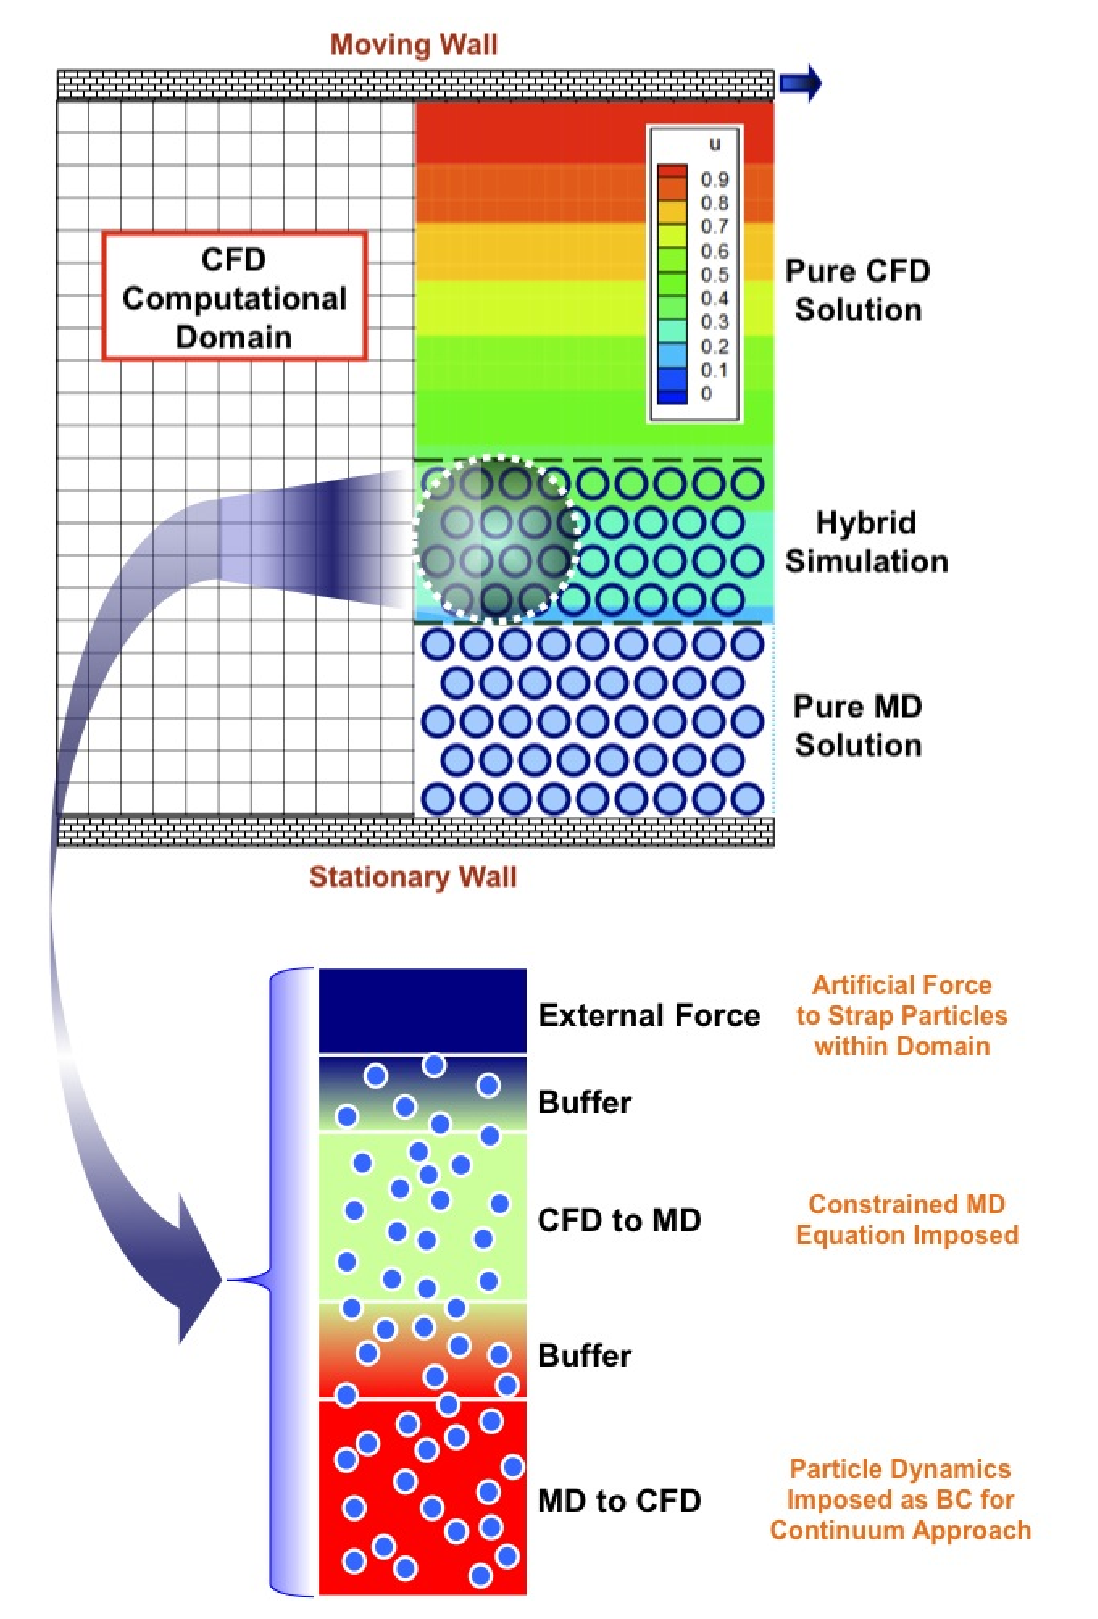
\includegraphics[scale=0.33]{fig1.eps}
%\linebreak
%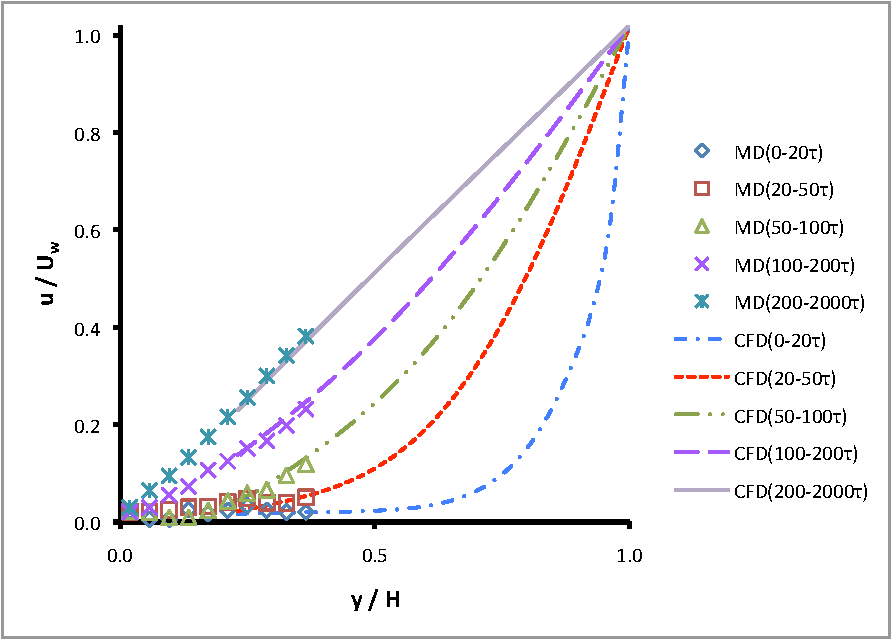
\includegraphics[scale=0.50]{Vel_Profile.PDF}
\caption{\small Schematic of CFD/MD Coupled Simulation of Channel Flow
  and the velocity profiles at different times}
\label{Fig:Couette}
\end{figure}
%%%%% FIGURE %%%%%

In this study, we based on the MPI version of the ``in-house''
incompressible CFD code~\cite{Lee} and the MPI version of
LAMMPS~\cite{LAMMPS} for MD. We had some modifications over these
application codes to implement hybrid schemes on each application
domain. In brief, the hybrid region where the coupling mechanism
between MD region and CFD region is executed comprises five
sub-regions. In the CFD boundary grid region positioned near the pure
MD region, velocities of particles obtained with MD are averaged and
used for boundary condition for the corresponding CFD computational
cells. The MD boundary zone is placed above the CFD boundary zone and
here, information on velocities from the CFD grid are imposed on
particles in the zone through dynamically constrained equation of
motion for MD. As illustrated in Fig.~\ref{Fig:Couette}, the coupling
mechanism is the key component for successful hybrid CFD/MD
simulations and our implementation follows the
literature~\cite{Nie},~\cite{Yen}.

% Between these zones, a buffer
% layer exists to avoid any harmful direct influences from one zone to
% another zone. The truncated and shifted Lennard-Jones potential is
% used for interactions of particles in MD simulation.

% To check the validity of the hybrid CFD/MD simulation, sudden-start
% Couette flow was employed that is similar to the test case used by
% O'Connell and Thompson~\cite{Thompson}.  The velocity profiles of
% hybrid approach are shown in the bottom of Fig.~\ref{Fig:Couette}. The
% line shows the velocity evolution which is solved by Navier-Stocks
% equations averaged over the given time intervals. MD results are shown
% as marks with same time intervals of CFD and overlap regions is
% indicated as both line and marks in the figure. These result is
% carried out for code validation of both CFD/MD and hybrid
% simulation. Good agreement between simulation results and analytical
% soluations.

As clearly indicated in Fig.~\ref{Fig:Couette}, the most prominent
computational challenge is how to run efficiently two separate stand
alone applications while efficiently conducting information exchange.
In other words, the time-to-solution is heavily dependent upon whether
a runtime environment can provide, (i) low collective-waiting times
(arising from batch queue wait times), and (ii) prevent an imbalances
in time to reach information exchange steps between the two codes. The
imbalance arises due to different performance between two distinctly
heterogeneous applications, CFD and MD, resulting in an unavoidable
time gap between arrival times of CFD and MD for the exchange step. We
propose to address this using dynamical resource allocation mechanism
with a load-balancing mechanism. In that sense, our SAGA-based
framework provides a single efficient runtime environment for the
coupled simulation.

%\Nkimnote{ }
%-------------------------------------------------------------------------
\section{SAGA and SAGA-based Frameworks for Large-Scale and Distributed Computation}

The Simple API for Grid Applications (SAGA) is an API standardization
effort within the Open Grid Forum (OGF)~\cite{ogf_web}, an
international standards development body concerned primarily with
standards for distributed computing. SAGA provides a simple,
POSIX-style API to the most common Grid functions at a sufficiently
high-level of abstraction so as to be 
independent of the diverse and dynamic Grid environments. The SAGA
specification defines interfaces for the most common Grid-programming
functions grouped as a set of functional packages
(Fig.~\ref{Fig:SAGA1}). Some key packages are:

\begin{figure}
%[!ht]
 \begin{center}
     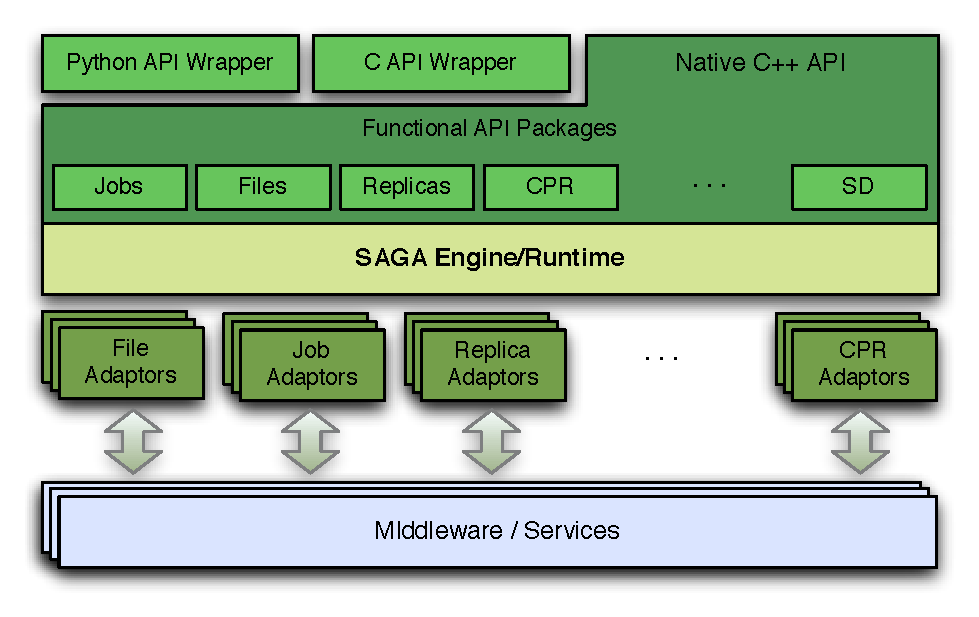
\includegraphics[width=0.40\textwidth]{stci_saga_figures-1.pdf}
 \end{center}
\caption{\small Layered schematic of the different components
  of the SAGA landscape. At the topmost level is the simple integrated API which provides the basic functionality for distributed computing. Our BigJob abstraction is built upon this SAGA layer using Python API wrapper} \label{Fig:SAGA1}
\end{figure}

\begin{itemize}
\item File package - provides methods for accessing local and remote
 filesystems, browsing directories, moving, copying, and deleting
 files, setting access permissions, as well as zero-copy reading and
 writing
\item Job package - provides methods for describing, submitting,
 monitoring, and controlling local and remote jobs. Many parts of
 this package were derived from the largely adopted
 DRMAA % ~\cite{drmaa_url}
 specification.
\item Stream package - provides methods for authenticated local and
 remote socket connections with hooks to support authorization and
 encryption schemes.
\item Other Packages, such as the RPC (remote procedure call) and Replica
 package
\end{itemize}


% \skonote{Introduction of PilotJob and BigJob (1 or 2 paragraphs) :
%   What is PilotJob, BigJob / what have been done so far and how
%   effective it was when using BigJob}

% \skonote{Joohyun, can you check this paragraph and improve it? In
%   this paragraph, I was going to talk about 'Structure and
%   Simulation Flow of BigJob Abstraction for Coupled Simulation'.}

Fig.~\ref{Fig:BigJob_Structure} shows the structure of BigJob and its
operation flow. When a BigJob is submitted to the remote resource, the
application manager monitors the status of this pilot-job through the
advert service. When resources are allocated to the BigJob, the
application manager divides obtained resources to its sub-jobs and a
coupled simulation starts under the control of a multi-physics agent
in the remote resource. Advert service keeps on getting the status of
a pilot-job from the queuing system and the status of sub-jobs from
multi-physics agent, also delivering these information to the
application manager by a push-pull mechanism. The application manager
watches the status of sub-jobs and decides the next event when the
coupled simulation is finished. When one default BigJob is launched,
sub-jobs keeps running until final solution is achieved and the
manager quits the pilot-job at that time. In cases multiple BigJobs
are submitted for the same simulation or a load balancing function is
included, sub-jobs experience several restarts from their
checkpointing data, reflecting changed processor allocation to each
application. In former case, resource allocation to each sub-job
follows a pre-defined map according to the number of BigJobs allotted
to this simulation: In latter case, resource allocation to each
sub-job becomes dynamic according to its performance, to be discussed
in the next section.

%%%%% FIGURE %%%%%
\begin{figure}
\centering
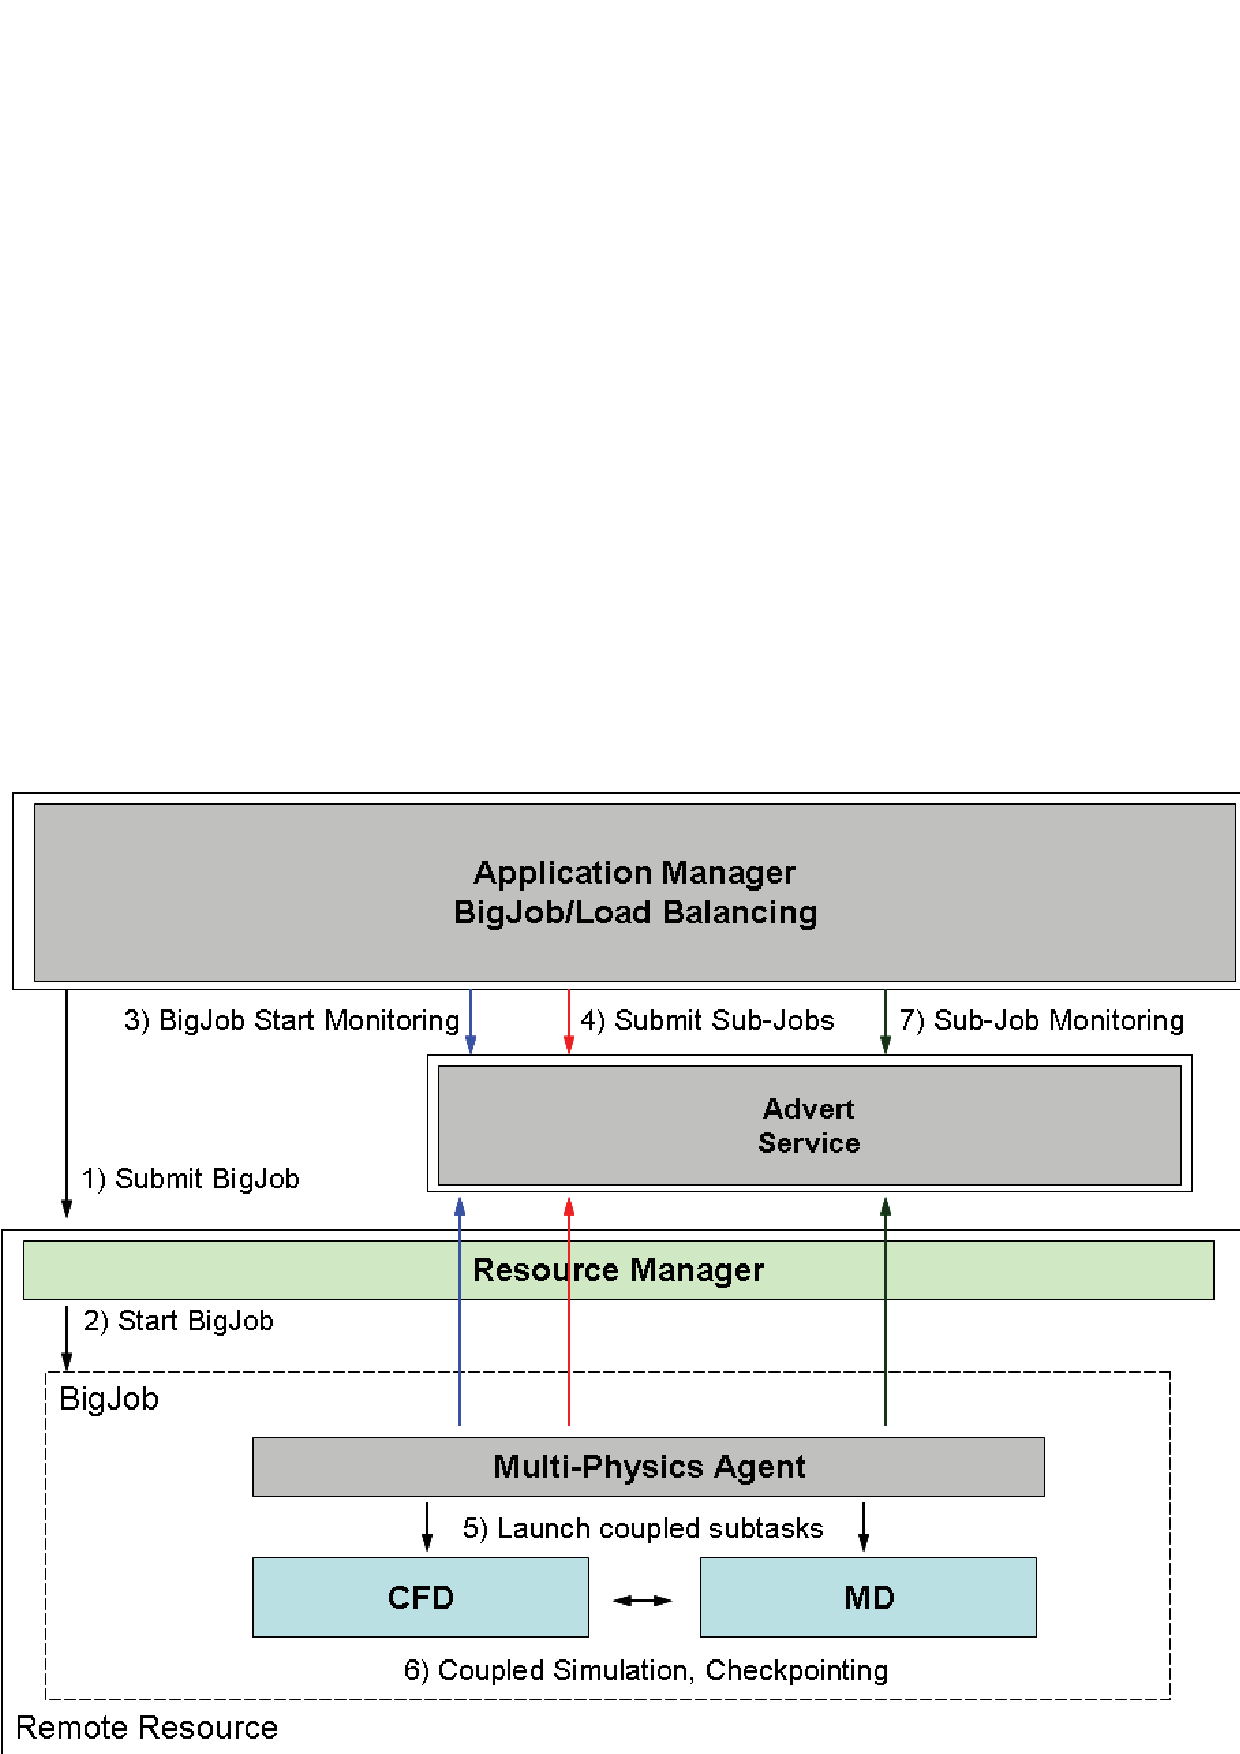
\includegraphics[scale=0.38]{Structure_of_BigJob}
\caption{\small Architecture of the Controller/Manager and Control
  Flow: Application manager is responsible for job management
  including BigJob and sub-job submission, their status monitoring
  functions. We implement a load balancing module, and migration
  service based on job information. Application agent system resides
  on each HPC resource and conducts job information gathering as well
  as communication with application manager via the advert service}
\label{Fig:BigJob_Structure}
\end{figure}
%%%%% FIGURE %%%%%

%-------------------------------------------------------------------------
\section{Load Balancing for Coupled Multi-Physics Simulation}

%\jhanote{ALL: Please use code, simulations and applications consistently through the paper.}

% SAGA and its pilot-job framework (BigJob) enable coupled, yet distinct
% simulations to be submitted to queuing system. This is done by submitting one container
% job, and re-distributing its processors to each task. Also, total
% execution time can further be reduced by assigning more BigJobs and
% dynamically reallocating resources to each sub-task with increased
% number of processors. However, the

% As the current simulation requires frequent data exchange between
% CFD and MD during the simulation, it is likely to increase
% communication cost (strictly, waiting time for communication in one
% application) if their loads are not well balanced, which is quite
% different from former BigJob application~\cite{Jha:2009} where data
% exchange takes place when sub-tasks stopped temporarily.

% Meanwhile, checking sub-tasks' performances and controlling their
% operation for load balancing runs counter to SAGA's philosophy of
% "using services without changing the application source". Thus, help
% from application side is necessary to employ a load balancing
% function on a BigJob.

The flexibility to re-distribute resources (processors) to the
individual task, does not imply efficient utilization. This is the
responsibility of a load-balancer (LB) We will discuss the
implementation and algorithm of this LB~\cite{Ko}; it is important to mention
that the LB functions in the context of the SAGA-BigJob framework.

Each application's load is determined by its elapsed time to run the
evolution loop. Here, time for initialization or inter-domain data
exchange are excluded from the counting, because they are one-time
event or irrelevant to application's performance.  The efficient
functioning of the LB is predicated on application codes being able to
restart from their checkpointing data effectively.  Also, application
codes should be equipped with generalized domain partitioning routine
to run a simulation with any number of processors, without harming
their parallel efficiency a lot. If above conditions are satisfied, it
makes sense to load the LB within the pilot-job, to implement dynamic
resource allocation between tasks.  Conceptually, the load-balancing
algorithm assigns more processors to a sub-task with greater runtime,
until two codes take the same wall-clock time between points when they
communicate. Interestingly, our approach is very simple and the
algorithm is indepenendent of applications upon which it is predicated
are, (1) each application code follows the ideal parallel efficiency.
(2) all processors in one node are assigned to one single task.

Let the computation time (between exchanges) of the two sub-jobs be
$t_{CFD}$ and $t_{MD}$, and the number of processors assigned to each
domain be $PE_{CFD}$ and $PE_{MD}$, respectively. Subscripts I and F
denotes initial and final states. Based on assumption (1), total
problem size of each application remains the same after the
re-allocation of resources,

\small
\begin{eqnarray}
W_{CFD}&=&PE_{CFD,I}\times t_{CFD,I}=PE_{CFD,F}\times t_{CFD,F} \nonumber \\
W_{MD}&=&PE_{MD,I}\times t_{MD,I}=PE_{MD,F}\times t_{MD,F}
\label{eq:SimTime_EachTask}
\end{eqnarray}
\normalsize
%\jhanote{Jeff: Please define what is $PE_{MD}'$, $t_{MD}'$} 

In spite of re-allocation, the total number of processor utilized
remains the same:

\small
\begin{equation}
%\begin{center}
PE_{TOT}=PE_{CFD,I}+PE_{MD,I}=PE_{CFD,F}+PE_{MD,F}
%\end{center}
\label{eq:PECondition}
\end{equation}
\normalsize

Our objective is to reduce the computation time of a sub-job until the
two application components show the same computation between the
exchange points, i.e., $t_{CFD,F} = t_{MD,F}$. From
Equation~\ref{eq:SimTime_EachTask} and Equation~\ref{eq:PECondition}
an optimal processors distributed for the CFD subtask would be:

\small
\begin{eqnarray}
PE_{CFD,F} & = & \frac {W_{CFD}} {(W_{CFD} + W_{MD})} \times PE_{TOT}
\end{eqnarray}
\normalsize

The MD simulation (sub-job) will follow a similar expression.  The
optimal processor distribution from above equation will return a
non-integer value. Also, under the second assumption (which is the
policy of many supercomputing centers), any load-balancing determined
as above, will proceed in discrete values
%determined by the number of CPU cores in a node.
expressed as the multiples of the number of CPU cores in a node. We choose the nearest discrete number to our load balancing as the optimal number of processor on each application.

%\jhanote{the  following is unecessarily complex. Simplify! Please remove  everything and replace with one single sentence without any  formulas. None of these terms are ever used again, so no point  introducing terminology if never used again!!}

%When upper and lower bound of $PE{CFD,F}$ is defined as
%%\begin{boundval}
%$ N_{UNIT} \times S \le PE{CFD,F} \le N_{UNIT} \times (S+1) $
%%\end{boundval}
%with $S = int(PE_{CFD,F} / N_{UNIT})$, either bound is going to
%satisfy optimal processor distribution between CFD and MD tasks. CFD
%computation time will determine coupled simulation time in the lower
%bound ,whilst simulation time in the upper bound is dependent on MD
%computation time, based on assumption (1). So, optimal processor
%distribution is the one which satisfies smaller computation time
%between $t_{CFD-in-Lower-Bound}$ and $t_{MD-in-Upper-Bound}$, who are
%expressed by
%\begin{eqnarray}
%t_{CFD-in-Lower-Bound} & = & \frac {W_{CFD}} {N_{UNIT} \times S}
%\nonumber \\
%t_{MD-in-Upper-Bound} & = & \frac {W_{MD}} {PE_{TOT}-N_{UNIT} \times (S+1)}
%\label{eq:Optimal_Time_Condition}
%\end{eqnarray}




%\hline
%\end{tabular}



%The control-flow within the BigJob Application-Manager when supporting a LB modules is shown in Fig.~\ref{Fig:BigJob_LB}. When one simulation loop is finished, the performance data of each subtask is sent to the load balancing module and it computes optimal resource distribution. Sub-job launcher restarts coupled application codes from their checkpointing data, according to the result of load balancing function. This process iterates until coupled simulation finalizes and processor allocation moves to the optimal condition during this process.

%%%%% FIGURE %%%%%
%\begin{figure}
%\centering
%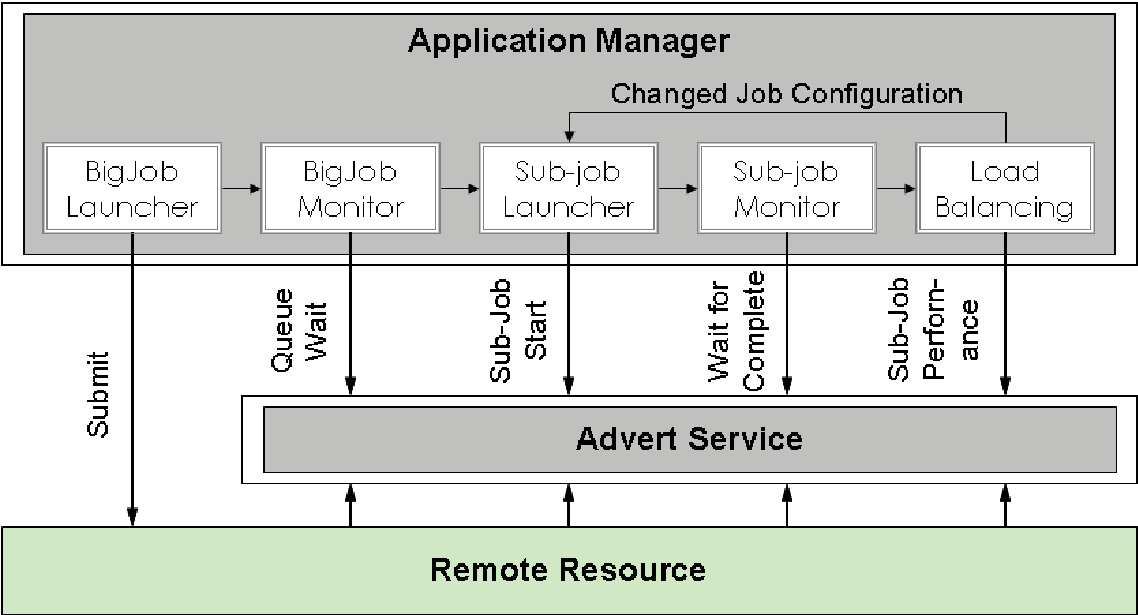
\includegraphics[scale=0.40]{BigJob_with_Load_Balance}
%\caption{\small Operation Flow of a BigJob with Load Balancing Function}
%\label{Fig:BigJob_LB}
%\end{figure}
%%%%% FIGURE %%%%%




%-------------------------------------------------------------------------
\section{Dynamic Resource Allocation for Coupled Simulations:
  Experiments and Analysis}

In Section 2, we outlined the challenges of running a coupled
multi-physics simulation using conventional queuing systems as the following: (i)
Difficulty of starting multiple applications concurrently; (ii)
Inability to balance the load among domains, and (iii) Fixed number of
allocated resources throughout the simulation. To address these
challenges we use the BigJob abstraction with a load balancing (LB) module
for dynamic resource allocation.

% \skonote{Need to check section 2, whether we have mentioned the
%   necessity of BigJob. This includes why we need BigJob, rather than
%   unifying application codes. Here, we should mention that 'minimizing
%   the application code change is the SAGA's great benefit'.}

% With the ultimate aim of reducing the total simulation time, we
% investigate acquiring idle resources during the simulation, by
% launching multiple BigJobs for one coupled simulation.

We outline three possible scenarios. In the first scenario, a single
BigJob is utilized to run the coupled simulations, with and without LB
(denoted as $S1_{LB}$ and S1 respectively) redistributing resources
based upon their individual performance.  In the second scenario (S2)
there are two BigJobs, and although they are started together, most
often one BigJob starts before the other; to increase efficiency, both
coupled simulations start with whatever resources are available as
part of the first (to run) BigJob. When the second BigJob becomes
active, there is a dynamic redistribution of tasks, such that the
larger of the two sub-jobs is assigned the bigger BigJob. Variant of
the above, when the two BigJobs are on two different machines forms
the third scenario (S3). In the remainder of this section we discuss
the details of these three different Use Cases.

% We compare the performance as measured by TTS using the benchmark
% case to be the situation when we do not have the ability to utilize
% the BigJob concept and thus each simulation interacts with the
% queueing system differently, and thereby each must be in an Active
% state before both can start running.

% \jhanote{please be sure to use co-scheduling where appropriate and
%   not concurrency}

%
%\skonote{Included a new subsection, to describe how the experiments are performed.}

% \subsection{Description of Experiments}
% A simple couette flow, which is depicted on Figure 1 in Section 2,
% is simulated to validate the runtime reduction by applying BigJob
% abstraction on CFD-MD coupled simulation. The current flow system is
% composed of 62,400 mesh points in CFD side and 23,188 particles in
% MD side, both of which are such a small system in each scientific
% domain. This coupled simulation runs for 2500 $$\tau$$ physical time
% to get a converged solution, which is equivalent to 25,000
% iterations on CFD code and 500,000 iterations on MD code. During the
% simulation, both codes update their boundary values by exchanging
% their simulation data through file-based approach, once in every 10
% $\tau$. This leads to 250 times synchronization between two
% application domains throughout the simulation.  A coupled simulation
% by the default one BigJob does not require any change of application
% codes. On the other hand, it is inevitable to have application codes
% changed to use advanced functions such as the load balancing between
% coupled codes or to get assigned with more resources during
% simulation, because SAGA does not have any control over application
% sides. First, in both cases, application codes need to have an
% application-level checkpointing and generalized domain partitioning
% method with any number of processor allocation. As the new resource
% assignment between two domains by a load balancing function or a new
% BigJob allocation can be applied when the simulation is temporarily
% stopped, application codes need to stop several times and restart
% from its checkpointing data with changed number of processors
% assignment. In the current test, application codes stop and restart
% from checkpointing data on every 500 $\tau$, which is the same as
% 1/5 of total iterations. Second, to use a load balancing function,
% application codes need to return their actual computation time data
% to the BigJob. This is far different from each application's
% simulation time, which can be monitored by the BigJob: One-time
% event such as domain partitioning or checkpointing, and waiting time
% between application domains which is going to be minimized as they
% are well-balanced, should be excluded from the consideration of
% application's performance. In the current test, CFD and MD codes
% have several time checking functions inside to capture total
% iteration time without inter-domain information exchange.  All these
% tests were conducted on supercomputing resources on LONI (Louisiana
% Optical Network Initiative)~\cite{LONI_web} resources and their
% specifications are listed on table~\ref{table:LONI_resource}. As
% given on the table, QueenBee system is far larger than other
% resources in total number of processors, while all the others are
% identical. Based on our monitoring over these systems, QueenBee has
% been very crowded while all others have been less occupied. Thus,
% tests on small systems are focused on quantifying runtime reduction
% by using the BigJob abstraction, while tests on QueenBee is rather
% involved in arguing the benefit of co-scheduling on crowded
% systems. wall-time limit is set to be 6 hours in all tests, which
% seems enough for the active simulation and inactive idling, i.e.,
% the time between the first job and second job allocations in
% conventional job submission.

\subsection{Description of Experiments}

Figure~\ref{Fig:OneBJ_Flow} shows two different scenarios: the first
(leftmost) shows the time evolution of a coupled simulation with the
conventional job submission and through one BigJob. In a conventional
way, individual tasks with resource requirements of $PE_{CFD}$ and
$PE_{MD}$, respectively, are independently submitted to the
conventional queuing system and job scheduler recognizes these coupled
tasks as two distinct jobs. Thus, they are going to start at a
different time, except when enough resources are available. In this
case, both tasks wait on the queue when no job is allocated, the first
allocated job idles to do data exchange with its counterpart, and run
actual simulation after both jobs are allocated. On the other hand, in
S1, a BigJob of size $PE_{CFD}+PE_{MD}$
is submitted to the queue, and coupled simulation directly starts when the resource is assigned on this BigJob. Because of co-scheduling of sub-jobs, a BigJob is free from a long inactive mode which is frequent in conventional job submission, while total runtime is the same if the resource distribution to sub-jobs is identical. However, eliminating
inactive mode does not guarantee total runtime is reduced,
because waiting to get one bigger allocation may happen to take more
than getting two allocations with smaller chunks. The same situation
can happen to the load-balanced case with one BigJob, which satisfies
the reduction of total runtime compared to other examples.
Figure~\ref{Fig:TwoBigJobs} illustrates scenarios S2 and S3 -- whereby
2 BigJobs are submitted as opposed to 1 BigJob. In S2 both BigJobs are
on the same machine, whilst in S3 they are on different machines.  As
we will show later, under certain load and queue conditions, it is
possible that two smaller BigJobs -- either S2 or S3, begin sooner
than a larger BigJob S1.

%%%%% FIGURE %%%%%
\begin{figure}
\centering
\includegraphics[scale=0.40]{Simulation_Time_of_One_BigJob.eps}
\caption{\small Comparison of dependencies encountered for
  coupled simulations submitted as conventional Jobs, to the scenario
  when using Pilot-Jobs (BigJob). Here we use only 1 BigJob. The
  conventional mode of submission experiences three phases of queue
  waiting (all jobs are waiting: $t_1-t_0$), inactive mode (one job is
  waiting for another: $t_2-t_1$), and active running (running a
  coupled simulation: $t_f-t_2$). On the other hand, inactive mode
  disappears when coupled simulation runs within one BigJob, as an
  allocated BigJob distributes its resource to sub-jobs.}
\label{Fig:OneBJ_Flow}
\end{figure}
%%%%% FIGURE %%%%%


% While we investigate the benefit of co-scheduling and load balancing
% on coupled distinct tasks in a single BigJob scenario, which is
% rather inclined to efficiently utilizing the computing environment
% within system's default configuration, we rather focus on physically
% increasing system's usage in next scenarios.  \skonote{Prof.Jha, can
%   you correct the above sentence? Intention was, 'while one BJ uses
%   computers efficiently within default system setup like queueing,
%   using two or more BJs will increase real usage of CPUs, thus
%   maximizing the use of idling resources.'}



% runtime environment for coupled multi-physics simulations would
% benefit from dynamic resource availability exploited by BigJob
% implementation. It is possible to assign more CPUs for a slowing
% application when another BigJob becomes available.  Compared to S1
% for a coupled simulation in Figure~\ref{Fig:OneBJ_Flow}, faster
% start of coupled subtasks. Also, when next BigJob is also allocated
% to this coupled simulation, total job size will be the same as one
% BigJob submission. Resource allocation and simulation flow is
% identical to the conventional job submission, but inactive idling in
% a conventional case disappears as a BigJob framework starts coupled
% subtasks with smaller number of processors when first job is
% allocated. So, submitting two BigJobs guarantees the reduction of
% total simulation time compared to conventional job submission, if
% all conditions are identical. If this two BigJob submission is
% applied on multiple sites, it is more likely to get two allocations
% faster than requesting two jobs in the same site. However, faster
% launch of two BigJobs does not guaranteed save of total simulation
% time, because time for data exchange between applications will also
% increase if distributed resources cooperate.


%%%%% FIGURE %%%%%
\begin{figure}
  \centering \includegraphics[scale=0.40]{Simulation_Time_of_Two_BigJobs.eps} \caption{\small
    Schematic comparing the distribution of simulations when 2 BigJobs
    are used, first on the same physical machine, then on different
    (distributed) machines. In both cases, coupled sub-jobs start
    running when the first BigJob is allocated at $t=t_1$ and
    experience resource reallocation with increased amount when the
    next BigJob becomes available. When two BigJobs are allocated,
    each sub-job occupies one BigJob and data exchange between jobs
    takes place across BigJobs.}  \label{Fig:TwoBigJobs} \end{figure}
%%%%% FIGURE %%%%%

We investigate a simple couette flow (Fig.~\ref{Fig:Couette}) as the
representative physical problem, to validate the performance gains and
resource flexibility of above scenarios.
%arising from the Pilot-Job based approach.
%by applying BigJob abstraction on CFD-MD coupled simulation.
The current flow system is
composed of 62,400 mesh points (CFD) and 23,188 particles (MD).
% both of which are such a small system in each scientific
% domain. 
In order to reach convergence, the coupled simulation runs for a
physical time of 2500$\tau$, which is the time unit related to the
characteristics of molecules. This is equivalent to 25,000 CFD
iterations and 500,000 MD integration steps. During the simulation,
both codes components update their boundary values by exchanging their
numerical data via files, once every 10 $\tau$. This leads to 250
synchronization steps between two simulation components over the
course of a single simulation run. For a rigorous test of a load
balancer, larger coupled simulation task (which has 150 times more
workload on CFD domain and 50 times on MD) also has been
experimented. 

No changes in the application codes were required in order to utilize
the BigJob capabilty; however, in order to utilize load-balancing
features or dynamic-resource assignement the application codes need to
be equipped with the ability to carry out application-level
checkpointing.  The application codes in addition to having
application-level checkpointing need generalized domain partitioning
method to work with a range of processor counts. In the current work,
the application codes experience five launch/re-launches (25 times in
larger simulation) to get assigned with changed number of processors,
either by the result of load balancing or more resource allocations.
%The wall-time limit of all simulations are set to 6 hours, which is large enough to encounter both the active and inactive phase experienced in conventional job submission. In the larger simulation, wall-time limt is increased to 24 hours, considering its runtime which is around 11 hours.

% A coupled simulation by the default one BigJob does not require any
% change of application codes. On the other hand, it is inevitable to
% have application codes changed to use advanced functions such as the
% load balancing between coupled codes or to get assigned with more
% resources during simulation, because SAGA does not have any control
% over application sides. 

% For example, with a new resource assignment, 
% a load balancing function or a new BigJob allocation can be
% applied when the simulation is temporarily stopped, application codes
% need to stop several times and restart from its checkpointing data
% with changed number of processors assignment. 

The use of a load balancing function requires one more change on
application codes. As load balancer refers to the performance data
from application codes, application codes need to return their actual
runtime, which excludes idle waiting on inter-domain
information exchange. This can be implemented by checking elapsed time
on inter-domain data exchange and subtracting it from total iteration
time.
%\jhanote{I'm not  sure I understand the following}
%One-time event such as domain partitioning or checkpointing, and waiting time between application domains which is going to be minimized as they are well-balanced, should be excluded from the consideration of application's performance.
%e architected the CFD and MD codes to have several time checking functions inside to capture total iteration time without inter-domain information exchange.


\skonote{Load factor definition and the way of testing: you can either edit this one or use the former one behind (which is commented out)}
Evaluation of a BigJob as a faster time-to-start solution requires the elaborative experiments with different processor requests and different wall-time limit on various system conditions. To quantify the waiting time of job submissions and analyze the variation of waiting time with system's conditions, we define the load-factor as the ratio of the number of active nodes to the total number of nodes on the machine; we testify the effect of load-factor on queue waiting time by submitting a number of experiments to the resources and monitoring the variance of load-factor at the submission and at the allocation time. Our experiments include multiple job submissions ranging from 8 to 64 processors with wall-time limit from 1 to 12 hours. This waiting time issue is also discussed by simulating above coupled simulations, in a way of submitting a BigJob and two conventional jobs concurrently and counting total waiting time in both cases. Both small and large simulations are conducted using 64 processors for a coupled task and wall-limit time is set to be either 6 hours or 24 hours, depending on their computation times.
%The load-factor is defined as the ratio of the number of active nodes to the total number of nodes on the machine; we measured this ratio at the instant when the job was submitted to the queuing-system, as well as when the job execution began, to correct for large variation in loads. The load-factor was recorded on every job submission while changing the requested number of processors from 8 to 64 and the requested wall-time limit from 1 hr to 12 hrs. The order of job execution depends on a variety of parameters such as submission time, backfill opportunities, number of actively scheduled jobs and queue priority including credential, fairshare, resource and service priority. The result of waiting time on the queue shows very diversity and variance as a matter of course.


Simulations used to validate and determine the performance measures were
conducted on supercomputing resources on TeraGrid machines (62,976
cores Ranger), shared TeraGrid-LONI (Louisiana Optical Network
Initiative)~\cite{LONI_web} machines (5,440 cores QueenBee)
and some smaller LONI machines such as Eric, Oliver, Louie and
Poseidon(512 cores each).  We monitored the load on these systems over a
long period of time (several weeks) and found Queenbee to be
significantly more loaded than other resources.

% \jhanote{Do we still want the following sentence?} Thus, tests on
% small systems focus on quantifying computation time reduction by using the
% BigJob abstraction, while tests on QueenBee is rather involved in
% arguing the benefit of co-scheduling on crowded systems.

% \jhanote{I don't understand the next sentence:} 
% monitoring over these systems, QueenBee has been very crowded while
% all others have been less occupied.

\subsection{Using Pilot-Jobs to submit Coupled Simulations:
  Performance Analysis}
  
%The load-factor is defined as the ratio of the number of active nodes to the total number of nodes on the machine; we measured this ratio at the instant when the job was submitted to the queuing-system, as well as when the job execution began, to correct for large variation in loads. The load-factor was recorded on every job submission while changing the requested number of processors from 8 to 64 and the requested wall-time limit from 1 hr to 12 hrs. The order of job execution depends on a variety of parameters such as submission time, backfill opportunities, number of actively scheduled jobs and queue priority including credential, fairshare, resource and service priority. 
% The result of waiting time on the queue shows very diversity and variance as a matter of course.




%The result of waiting time on the queue shows very diversity and variance as a matter of course.

\begin{table}[t]
  \caption{\small  Effect of various configurations on waiting
time. The tables show the actual waiting time on the queue with
respect to the changing number of processors and different wall-time
limits when jobs were submitted on Ranger and Queenbee.  Comparing the
actual waiting time with the number of processors on each wall-time
limit, quantitative tendency of waiting times is to somewhat decrease
when requested number of processors increases. But the relationship
between the waiting time and wall-time limit was hardly observed.
However, these works constitute a good case study for showing variance
of actual waiting time on the queueing system.}
\label{table:waitingtime}
\centering
\begin{tabular}
{p{0.4in} || p{0.4in} p{0.4in} p{0.4in} p{0.4in} p{0.4in}}
\multicolumn{6}{c}{\phantom{\tiny 100}}\\
\hline
%\midrule
 \multirow{3}{0.4in}{Number of processors}&
 \multicolumn{5}{c}{Requested wall-time at 92$\pm$6\% load (Ranger)}
\\
\cline{2-6}
%\cmidrule{2-6}
 & \nyc 2hr
 & \nyc 3hr
 & \nyc 4hr
 & \nyc 6hr
% & \nyc 6hr
& \multicolumn{1}{c}{12hr}
%  &1hr &2hr &4hr &6hr &12hr
\\
\cline{2-6}
%\cmidrule{2-6}
 &\multicolumn{5}{c}{Waiting time on the queue [sec]}
\\
\cline{1-1}
%\cmidrule{1-1}
\nyc 16
 & \nyc 9989 & \nyc 15984 & \nyc 39151 & \nyc 65 & \multicolumn{1}{c}{66}
\\
\nyc 32
 & \nyc 15371 & \nyc	4106 & \nyc 11376 & \nyc 54 & \multicolumn{1}{c}{55}
 \\
\nyc 48
  & \nyc 13264 & 4392 \nyc  & \nyc 37780 &\nyc 43 & \multicolumn{1}{c}{44}
\\
\nyc 64
 & \nyc 9944 &	\nyc 1975	 & \nyc 39855 & \nyc 31 & \multicolumn{1}{c}{32}
\\
\hline
%\midrule


\multicolumn{6}{c}{\phantom{100}}\\
\hline
%\midrule
 \multirow{3}{0.4in}{Number of processors}&
 \multicolumn{5}{c}{Requested wall-time at 95$\pm$4\% load (Queenbee)}
\\
\cline{2-6}
%\cmidrule{2-6}
 &\nyc 2hr
 &\nyc 3hr
 &\nyc 4hr
 &\nyc 6hr
 &\multicolumn{1}{c}{12hr}
\\
\cline{2-6}
%\cmidrule{2-6}
 &\multicolumn{5}{c}{Waiting time on the queue [sec]}
\\
\cline{1-1}
%\cmidrule{1-1}
\nyc 16
 & \nyc 14339 & \nyc 3578  & \nyc 39113 & \nyc 6 & \multicolumn{1}{c}{940}
\\
\nyc 32
 & \nyc 14312 & \nyc 3550 & \nyc 39238 & \nyc 5 &\multicolumn{1}{c}{6344}
 \\
\nyc 48
 & \nyc 21555 & \nyc 3517 & \nyc 39207 & \nyc 4 & \multicolumn{1}{c}{6353}
\\
\nyc 64
 & \nyc 21541 & \nyc 3489 & \nyc 39179 & \nyc 3 & \multicolumn{1}{c}{6329}
\\
\hline
%\midrule
\end{tabular}
\end{table}

We wanted to see if we could come up with an analysis that would tell
us how running larger and/or longer simulations effects the actual
waiting time on the queue. What we did was the following. We chose two machines with more than
5000 processors, Ranger and Queenbee. We submitted jobs of different
sizes, requiring different wall-time limits. Each time we submitted a
job, we gathered the load-factor and the actual waiting time on the
queue. Lots of factors effect the waiting times. Most important of
them is the load at the moment on the machine, requested wall-time
limit and also the number of processors requested. Two more factors
that effect this are the backfilling that occurs when some other
irrelevant job ends and the changes in the priority of our own job
when a particular higher priority job joins the queue.  Also, the internal queueing policy of supercomputing centers may effect the waiting time on the queue based on  their queueing priority  including credential, fairshare, resource and service priority. The waiting
time has a tendency to decrease as the number of processors of a job
increase, as can be seen from Table~\ref{table:waitingtime}.
Considering only the data from the jobs which did not go through
backfilling, it can be seen that larger processor jobs start earlier
based on the priority of jobs. 

We cannot claim this just by running some tests on a couple of
machines. It may be, in part, due to the policies and loads under
which a particular machine is run. The waiting time has a little
relationship with wall-time limit of jobs. But from experience, we
feel that running a large job is better than running two smaller
jobs. We say that the sum total of the waiting times of two smaller
jobs is going to be larger than the waiting time of a single large
processor job. This is especially true in cases where the jobs need to
interact, as shown in Fig.~\ref{Fig:OneBJ_Flow}.

%The order of job execution depends on a variety of parameters such as submission time, backfill opportunities, number of actively scheduled jobs and queue priority including credential, fairshare, resource and service priority. 

The result of time-to-start on conventional job submissions and a single BigJob launch is presented in Table~\ref{table:BJwaiting}. Test results do not exactly coincide with our waiting time experiments in every test. In the larger simulation problem which has longer wall-time limit, the result follows our former experiments that a BigJob has the potential of faster time-to-start than two conventional submissions. On the other hand, a small problem resulted in the faster time-to-start in conventional case. 
%there is no guarantee whether two smaller job submissions would utilize backfilling capability more effectively or one BigJob launch will get the benefit of higher priority by resources' queueing policy. According to the experiments presented in 
Meanwhile, the large standard deviation of the resultant data leaves much to debate on the reliability of these data. At least, it is clear that a BigJob submission eliminates the possibility of simulation's failure due to long inactive phase, which shall cause far longer wall-time limit setup than actual runtime.

%, though the result gives conventional job submission showed faster start in small wall-time limit and BigJob had better with longer wall-time limit, the large standard deviation leaves much to debate on the reliability of these data. The only thing clear is that a BigJob submission eliminates the possibility of simulation's failure due to long inactive phase, which shall cause far longer wall-time limit setup than actual runtime.

\begin{table}[t]
\caption{\small  Waiting and inactive time on conventional job submissions and a single BigJob submission. In both cases, conventional job is submitted to use 2$\times$32 processors and a BigJob requests 64 processors. Conventional job showed faster time-to-start (i.e., the sum of waiting time and inactive mode) on small problem size with 6 hours of wall-time limit, while a BigJob gets allocated faster with longer wall-time limit. Conventional job submission showed 3 failures during the test due to the timeover of wall-time limit in the first-started job. Experiments were conducted on small and less crowded LONI clusters.}

\label{table:BJwaiting}
\centering
\begin{tabular} {p{0.55in} || p{0.7in} p{0.7in} p{0.7in}}
\multicolumn{4}{c}{\phantom{\tiny 100}}\\
\hline
 \multirow{2}{0.55in}{}&
 \multicolumn{3}{c}{Small simulation with 6 hrs wall-time limit} 
\\
\cline{2-4}
 & \nyc Waiting time
 & \nyc Inactive mode
 & \multicolumn {1}{c}{Failed runs}
\\
 \hline
   \nyc Conventional & \nyc 12318$\pm$15649 & \nyc 7407$\pm$11375 & \multicolumn {1}{c}{2} \\
  \nyc 1 BigJob & \nyc 29452$\pm$31946 & \nyc 0 & \multicolumn {1}{c}{0} \\
 \hline

\multicolumn{4}{c}{\phantom{100}}\\
\hline
 \multirow{2}{0.55in}{}&
 \multicolumn{3}{c}{Large simulation with 24 hrs wall-time limit} 
\\
\cline{2-4}
 & \nyc Waiting time
 & \nyc Inactive mode
 & \multicolumn {1}{c}{Failed runs}
\\
\hline
 \nyc Conventional & \nyc 83102$\pm$77134 & \nyc 47488$\pm$55647 & \multicolumn{1}{c}{1}
\\
 \nyc 1 BigJob & \nyc 76645$\pm$55474 & \nyc 0 & \multicolumn{1}{c}{0}
\\
\hline

\end{tabular}
\end{table}



\subsection{Scenario S1: Pilot-Job with Load Balancing}

%\jhanote{Do not have such long paragraphs. One paragraph should
%  represent one simple compact idea. Maxm of 4-5 sentences!!}

Runtimes of the coupled simulation with a single BigJob is given on Table~\ref{table:oneBJ_Test}. In both small and large simulations, a default BigJob task takes about 1 percent longer than the conventional test. This is reasonable because a default BigJob has the same processor distribution between sub-jobs as the conventional job, while BigJob has the overhead of sub-jobs' status monitoring and communication with advert server. In cases of load-balanced BigJob simulations, runtime is saved by about 13 percent compared to conventional tests. In the large problem, a load-balanced BigJob simulation relatively shows higher standard deviation due to the unexpected instability of a computing resource during one experiment, which is to be discussed in detail below.



\begin{table}[t]
%\setlength{\tabcolsep}{1pt}
%\begin{table}[!ht]
%\begin{center}
\caption{\small Results of runtime for S1, S1+LB and conventional submission. 6 distinct experiments were accomplished on each simulation. In both cases, S1 shows about 1\% overhead due to the communication with advert server. On the other hand, S1+LB tests show about 13\% runtime save compared to conventional submission. 64 processors are used on all simulations.}
\label{table:oneBJ_Test}
\centering
\begin{tabular} {p{0.5in} || p{0.7in} p{0.7in} p{0.7in}}
\multicolumn{4}{c}{\phantom{\tiny 100}}\\
\hline
 & \nyc Conventional
 & \nyc S1
 & \multicolumn{1}{c}{S1+LB}
\\
\hline
 \nyc Small sim. & \nyc 757$\pm$1.89 & \nyc 764$\pm$1.41 & \multicolumn{1}{c}{661$\pm$4.41} \\
 \nyc Large sim. & \nyc 39595$\pm$119.2 & \nyc 39906$\pm$206.3 & \multicolumn{1}{c}{34350$\pm$1302.7} \\
\hline
%\midrule
\end{tabular}
\end{table}
The validity of a load balancing function can be discussed by the
change of processor distribution between subtasks throughout the
simulation. In the result of a small simulation in
Fig.~\ref{Fig:LBSmall}, both CFD and MD subtasks are assigned with 32
processors initially. After two simulation loops, a load balancer
converges to the processor distribution of 12 to 52 between CFD and MD
jobs and this processor distribution remains the same until the
simulation completes. Runtime reduces from 153 seconds at the initial
stage to 107 seconds after the convergence. Total computation time is
596.19 seconds, which is different from 663 seconds counted from
BigJob application manager. This time difference implies that the
BigJob application manager spends about 13 seconds on executing its
internal commands including the run of a load balancing function and
sub-job re-launch.

%%%%% FIGURE %%%%%
\begin{figure}
\centering
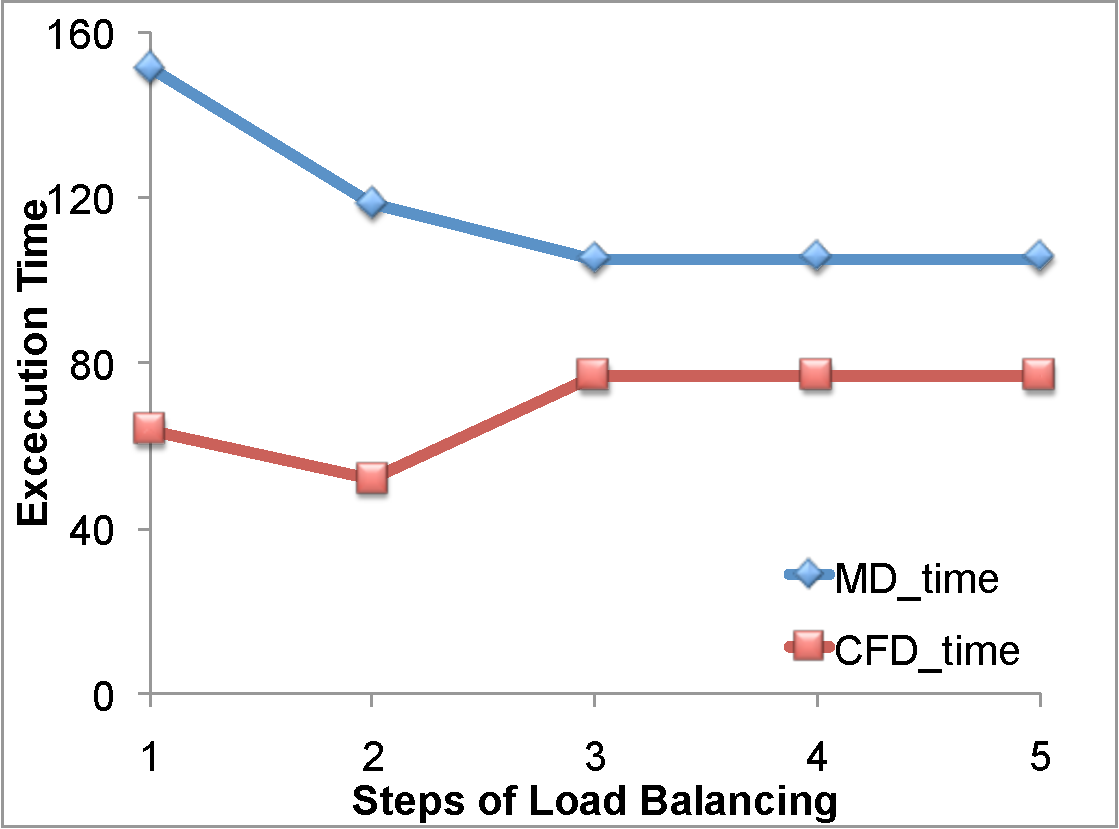
\includegraphics[scale=0.3]{fig6_1.pdf}
\linebreak
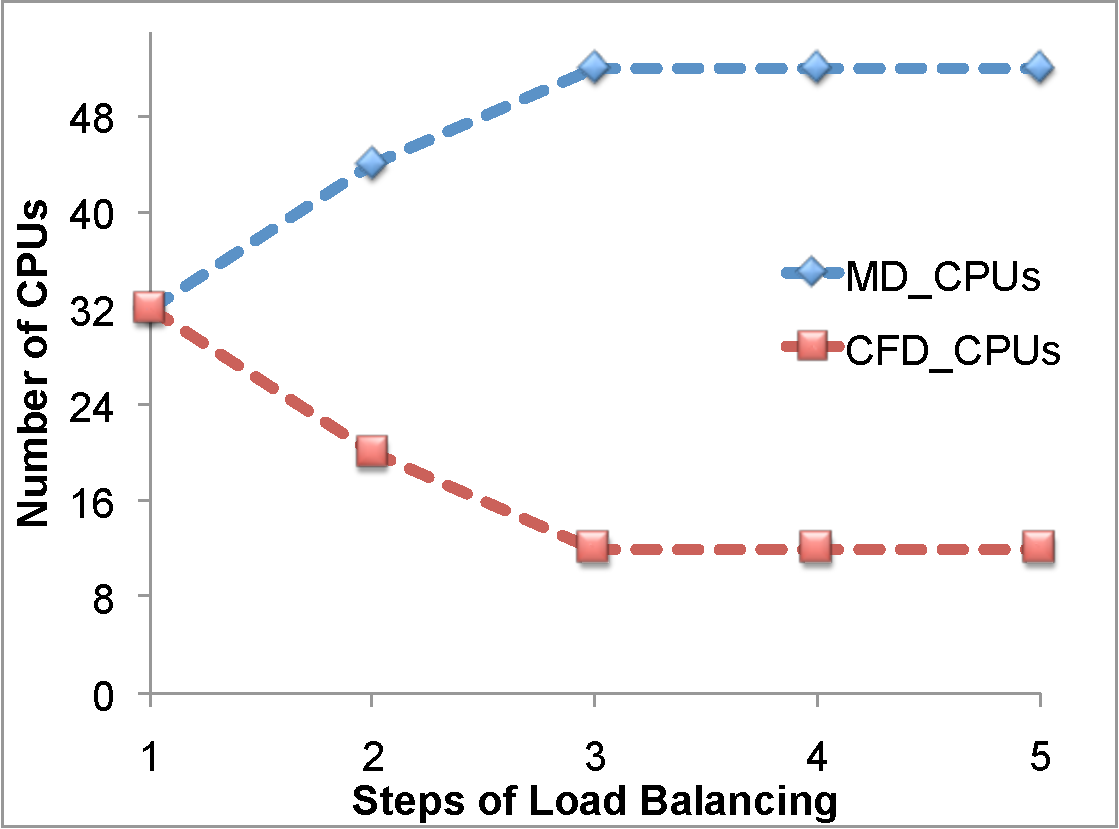
\includegraphics[scale=0.3]{fig6_2.pdf}
\caption{\small Change of processor distribution between CFD and MD
  jobs and resultant computation time in the small simulation. A load
  balancer starts from the same number of processors assigned to both
  sub-jobs and detects 20 to 44 processor distribution as the optimal
  solution. The poor scalability of CFD job makes the load balancer to
  search for the optimal condition once again and the processor
  assignment finally reaches to a steady solution of 12 to 52 between
  two sub-jobs. Computation time for every simulation loop reduces
  from 153 seconds to 107 seconds after the balancing.}
\label{Fig:LBSmall}
\end{figure}
%%%%% FIGURE %%%%%

The result of computation time evolution on a large simulation is seen
in Fig.~\ref{Fig:LBLarge}. On most experiments, which is given in the
left side of Fig.~\ref{Fig:LBLarge}, a load balancer directly goes to
a converged solution of processor distribution, which is 24 to 40
between CFD and MD jobs. On the other, in one experiment, computing
nodes assigned to MD simulation seem to have temporarily experienced
the internal overhead as shown from the right side of
Fig.~\ref{Fig:LBLarge}. This overhead temporarily increased MD
computation time a lot and a load balancer shows the fluctuating
pattern of processor distribution in response to this temporary
instability. A load balancer goes to a different steady solution after
the system settled down, which is the processor distribution of 20 to
44 between two sub-jobs. Compared to the steady solution in stable
cases, computation time for one simulation loop increases in this
processor distribution increases from 1320 seconds to 1380
seconds. This leaves the requirement of refining a load balancing
function, to predict more precisely on parallel performances of
application codes.


% %%%%% FIGURE %%%%%
\begin{figure}
\centering
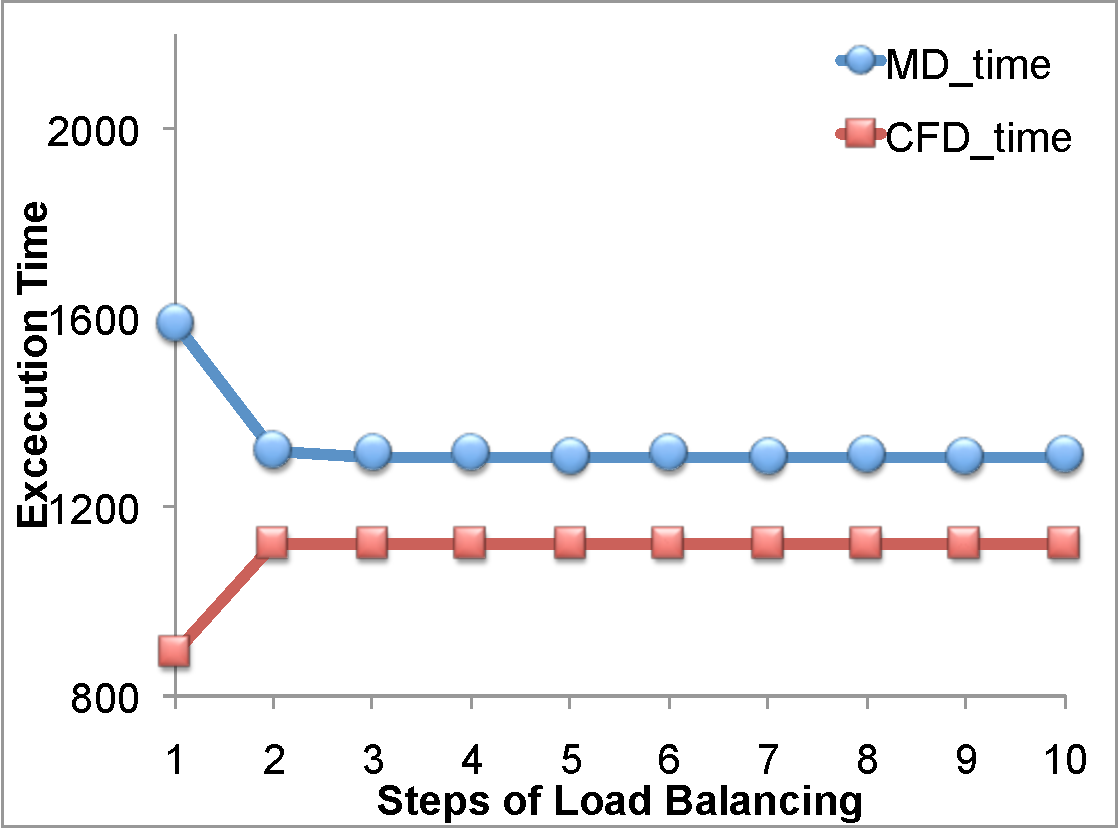
\includegraphics[scale=0.21]{fig7_11.pdf}
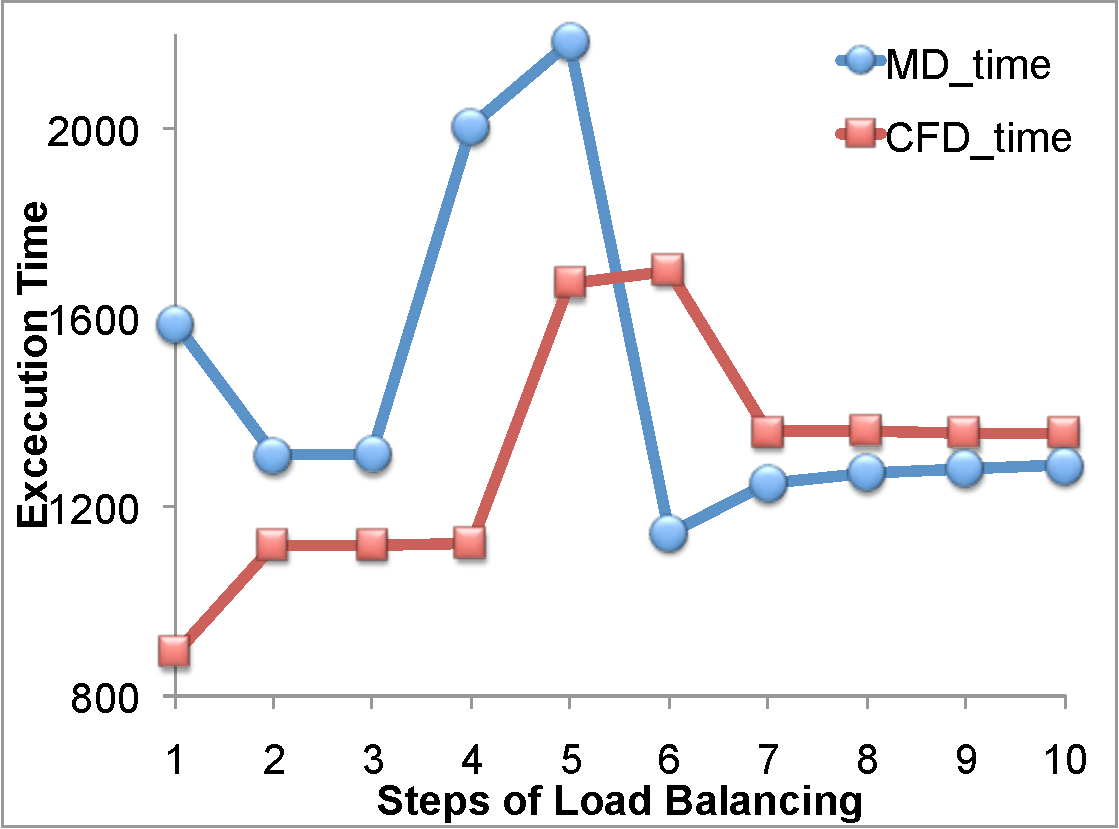
\includegraphics[scale=0.21]{fig7_21.pdf}
\linebreak
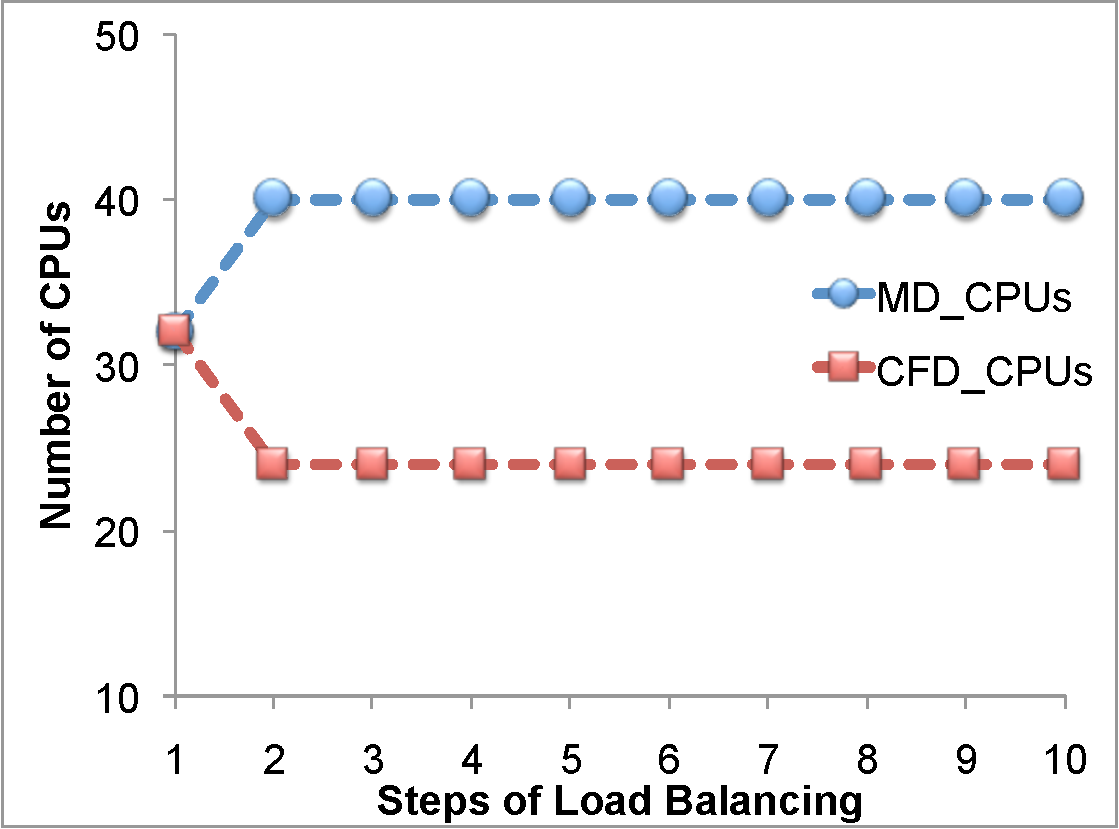
\includegraphics[scale=0.21]{fig7_12.pdf}
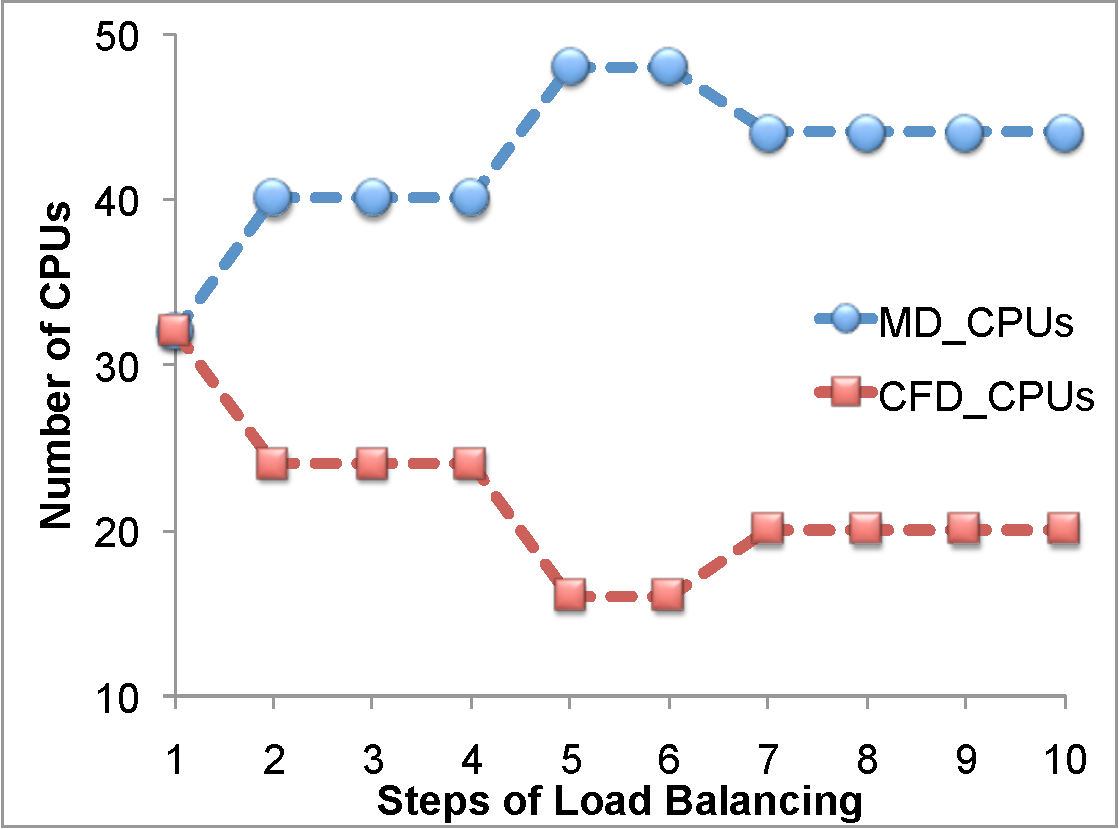
\includegraphics[scale=0.21]{fig7_22.pdf}
\caption{\small (Left Column) Change of processor distribution between
  CFD and MD jobs and resultant computation time in the large
  simulation. A load balancer directly finds the processor
  distribution of 24 to 40 between CFD and MD jobs and remains the
  steady state until it completes after 25 simulation loops. Initial
  computation time of 1605 seconds reduces to 1320 seconds after the
  convergence. (Right Column) Plots showing non-monotonic resource
  assignment by the LB, and thus demonstrating how the load balancer
  can be self-correcting and adapt to changing performance; after
  increasing the number of processors assigned to the MD, the
  load-balancer unassigns the additional processors.}
\label{Fig:LBLarge}
\end{figure}
%%%%% FIGURE %%%%%


%\jhanote{You need to really sit down and rewrite this. It is almost
%  impossible to understand anything here!!!}


\subsection{Scenario S2 and S3: Logically and Physically Distributed
  Pilot-Jobs}

In Table~\ref{table:TwoBigJobs}, results from the four test runs
representing scenarios S2 and S3 using two BigJobs are presented.  The
general setup for scenarios S2 and S3 is that when two BigJobs are
submitted, one BigJob becomes active first and the other BigJob
becomes available later -- either on the same resource (S2) or on
another resource (S3).  The MD and CFD request half of each
BigJob. When the second BigJob becomes active, each application is
immediately configured to run in each BigJob so as to consume all
BigJob cpus. Therefore, more cpus allow each application to speed
up. Conceptually the LB scheme adopted for S1 can be trivially applied
here, but for simplicity and as proof-of-concept, we confine our test
runs to the configuration in Fig.~\ref{Fig:TwoBigJobs}, i.e., without
a load balancing scheme to determine an optimal distribution of
resources.

As shown in the table, the results with these four test cases clearly
demonstrate performance gains with additionally available cpus when
two BigJobs.  The performance gain is examined with respect to two
components ${T_{comm}}$ and ${T_{compute}}$ of the total
time-to-solution.  % The major performance gain is indicated with a
% shorten ${T_{compute}}$. 
${T_{compute}}$ represents the maximum of (${T _{MD,compute}}$,
${T_{CFD,compute}}$) -- which is the longer compute time of two
applications, and%  Each $T_{app,compute}$, where ${app}$ is MD or CFD, is
% measured with 
by the start time and the end time between the data exchange.  As more
cpus become available with the incoming BigJob, more gain in the
performance is achieved as shown in the case of test 4.  On the other
hand, the time for communication, ${T_{comm}}$ is further decomposed
into ${T_{read-write}}$ and ${T_{file-transfer}}$.  Note that the
latter is only required with S3.  There are other components that
contribute to the overall time-to-solution, such as the waiting time
in queue etc., but are not considered here to focus on the performance
gain arising from simple dynamic execution (resource allocation) as
illustrated from S2 and S3.

% Performance gains with two BigJobs. Performance is measured with CPU
% times consumed by MD, since test cases we used always require longer
% CPU times for MD than those of CFD.  Performance gains with
% additionally available BigJob can be seen by comparing MD CPU times
% with those obtained with the initial BigJob.  Measurements were
% carried out with LONI cluster systems.  louie and poseidon are dell
% cluster systems having 128 nodes with 4 cores in a
% node. \jhanote{add BigJob size --- which 8 and 16} Test 1 and 2
% correspond to Use Case 2; Test 3 and 4 correspond to Use Case 3
% \newline }

% \jhanote{I think
%       we should revisit the way this is presented, i.e., the utility
%       of using the time of the MD phase?}  \Jkimnote{I got rid of MD
%       time as a measure since it causes unnecessary confusion}
%     \jhanote{this caption is tooooo long and needs simplifying. Too
%       many latex errors!} \jhanote{Look at all the wasted white
%       space!!! We are running short of space. Fix}

\begin{table}[!h]
\begin{center}
  \caption{\small Performance measured for Scenarios S2 and S3 (2
    BigJobs on 2 different machines).  Here, we present the time to
    solution in terms of two components, ${T_{comm}}$ and
   ${T_{compute}}$.  The details on how to conduct these experiments
    are described in the text.  All measured time are in seconds.
    BigJob size refers to the size of two BigJobs as determined by the
    number of requested cpus. Resource describes the system used (L
    stands for Louie; P for Poseidon. L \& P are LONI resources) }
\label{table:TwoBigJobs}
\begin{tabular}{ c || c  c  c  c}
\hline
Test & 1 & 2 & 3 & 4  \\

\hline
Scenario & S2 & S2 & S3 & S3 \\
BigJob size & (8,16)  & (8,16) & (8, 16) & (16,32) \\
Resource & P  & L  &  L + P & L + P \\
\hline
1 BigJob &   & & & \\
${T_{compute}}$ & 1037.2& 1045.2 & 1049.0 & 534.2\\
${T_{comm}}$ & 0.006 & 0.010 & 0.912 & 0.957 \\
\hline
2 BigJob  &   & & & \\
${T_{compute}}$ & 277.2 & 277.8& 276.8 & 150.4 \\
${T_{comm}}$ & 0.041 & 0.009 &  0.990 & 0.60 \\
\hline
\end{tabular}
\end{center}
\end{table}

% \jhanote{The $T_{comm}$ has two components: $T_{read_write} +
%   T_{transfer}$. We need to determine the first component. We will not
%   be able to do so rigorously, but we need to show a good-faithed
%   attempt at deriving it.  The we need to determine the transfer
%   overheard, and find out if it is truly negligible when compared to
%   $T_{read_write}$. We need to also mention/determine if
%   $T_{read_write}$ is the same -- when using 2 different machines as
%   it is when using 1 machine. As would be expected.}

According to our results, the communication time is insignificant even
for S3 -- in part thanks to the small size of the data required to be
exchanged.  Of course, the file transfer depends heavily on the
network condition, but it is not expected to become a major issue
considering the observation that ${T_{comm}}$ is a tiny fraction of
${T_{compute}}$.  Furthermore, we expect that the ratio of the two
components will remain similar, or if anything become larger (i.e.,
${T_{comm}}$ become less significant) as the size of physical system
simulated increases, i.e., the number of particles in MD or the number
of mesh points increases.  Indeed, the development of an efficient
runtime environment for hybrid CFD/MD simulation lies in finding a way
to decrease ${T_{compute}}$.  Arguably, the results in the
table~\ref{table:TwoBigJobs} suggest that a BigJob-based runtime
environment is able to provide a reasonable solution to this end.

\section{Conclusions}

\jhanote{Conclusion needs fine scale adjustment} \jhanote{Place
  appropriately. This discusses why simple MPI generalizations are not
  enough.} Some of these problems arise from the nature of the
simulations: large scale simulations that would not be able to run
concurrently on the same resource, while others issues are quite
technical such as dynamic shrinking/expanding the number of MPI
processes of each application (dynamic load-balancing). Using MPI as a
coupling layer would also require code modification, adding
infrastructure to support simulation-to-simulation communication. To
maintain a high level of adaptivity, abstraction, interoperate between
various application codes, and to eliminate application code invasion,
we opted not to use MPI and focus on non-invasive abstract coupling
layers.

In this work, we report the first production-level framework that
enables an efficient runtime environment targeting the coupled
multi-physics application comprising MD and CFD as two coupled stand
alone applications...

It is not trivial to integrate a targeted scientific application with
a resource management system that is aware of the challenges arising
from the distributed computing as well as the local scheduler
implemented with the local resource management policy..

Overcoming the co-scheduling requirements and implementing dynamic
resource allocation mechanism were two main goals motivating a novel
development and our test runs demonstrated its potential for large
scale scientific simulations benefiting scientific problems that are
only tackled by a coupled hybrid MD-CFD calculation.  Our development
is built upon the BigJob framework enabled by the SAGA. ... simple and
consistent interface for managing HPC resources is easily achieved
resulting the agile and flexible development. We tested our
development for three cases and demonstrated its capability. In
addition, the use cases includes the usage of the Condor-glide-in as
our BigJob framework is closely related. ... Some of those are i)
employment of load balancing mechanism ii) advantages from
implementation of dynamic allocation in heterogeneous distributed
computing resources iii) simple solution for the co-scheduling
requirements for the coupled tasks.

We have established that the performance advantage of using BigJobs is
invariant with the size of the machine, i.e., small LONI machines such
as Eric, to the largest machines available such as Ranger. This is not
so much about the machine, but the system sizes of the physical-models
that we are investigating.

In summary, use of a BigJob will eliminate idling operation of a
subtask, which waits for another application to start running. Also,
employing a load balancing function will let coupled codes use
allocated resources more efficiently. Furthermore, using two BigJobs
promotes the reduction of total runtime, compared to conventional job
submission. Meanwhile, launch of two BigJobs does not intend to use
resources more efficiently than conventional job allocation, but
intend to save total computation time more than one BigJob test case,
by utilizing more available resources.

  % \jhanote{Notes: (i) (ii) Need to establish clearly how we are
  %   measuring the times in Table I. Are we using 'startq'? Remember
  %   enough details should be presented to make the experiments
  %   reproducible (iii) What is the largest system size that we can
  %   simulate using BigJob and/or using independent execution
  %   threads? (iv) What is the final ratio of $N_{MD} to N_{CFD}$? Is
  %   it always the same? How do we counter the argument that the
  %   final configuration can be determined with a few simple
  %   pre-processing runs? What is the importance of dynamic resource
  %   management, i.e. start with initial Configuration I and adapt to
  %   Final Configuration F with intermediate states in between?  }


\section*{Acknowledgment}
This work is part of the Cybertools (http://cybertools .loni.org)
project and primarily funded by NSF/LEQSF (2007-10)-CyberRII-01.
Important funding for SAGA has been provided by the UK EPSRC grant
number GR/D0766171/1 (via OMII-UK). This work has also been made
possible thanks to computer resources provided by LONI. We thank Andre
Luckow for initial work on BigJob, Lukasz Lacinski for help with SAGA
deployment (via HPCOPS NSF-OCI 0710874) and Joao Abecasis for his work
on the SAGA Condor adaptors.

%-------------------------------------------------------------------------
\nocite{ex1,ex2}
%\bibliographystyle{latex8}
\bibliographystyle{IEEEtran}
\bibliography{saga_tg08}


\end{document}


